\section{A Tour Through Tree RCU's Expedited Grace Periods}
\label{sec:rcu:A Tour Through Tree RCU's Expedited Grace Periods}


\subsection{Introduction}

This document describes RCU's expedited grace periods.
Unlike RCU's normal grace periods, which accept long latencies to attain
high efficiency and minimal disturbance, expedited grace periods accept
lower efficiency and significant disturbance to attain shorter latencies.

There are two flavors of RCU (RCU-preempt and RCU-sched), with an earlier
third RCU-bh flavor having been implemented in terms of the other two.
Each of the two implementations is covered in its own section.


\subsection{Expedited Grace Period Design}

The expedited RCU grace periods cannot be accused of being subtle,
given that they for all intents and purposes hammer every CPU that
has not yet provided a quiescent state for the current expedited
grace period.
The one saving grace is that the hammer has grown a bit smaller
over time:
The old call to \co{try_stop_cpus()} has been
replaced with a set of calls to \co{smp_call_function_single()},
each of which results in an IPI to the target CPU\@.
The corresponding handler function checks the CPU's state, motivating
a faster quiescent state where possible, and triggering a report
of that quiescent state.
As always for RCU, once everything has spent some time in a quiescent
state, the expedited grace period has completed.

The details of the \co{smp_call_function_single()} handler's
operation depend on the RCU flavor, as described in the following
sections.


\subsection{RCU-preempt Expedited Grace Periods}

\co{CONFIG_PREEMPTION=y} kernels implement RCU-preempt.
The overall flow of the handling of a given CPU by an RCU-preempt
expedited grace period is shown in the following diagram:

\begin{center}
\resizebox{.6\columnwidth}{!}{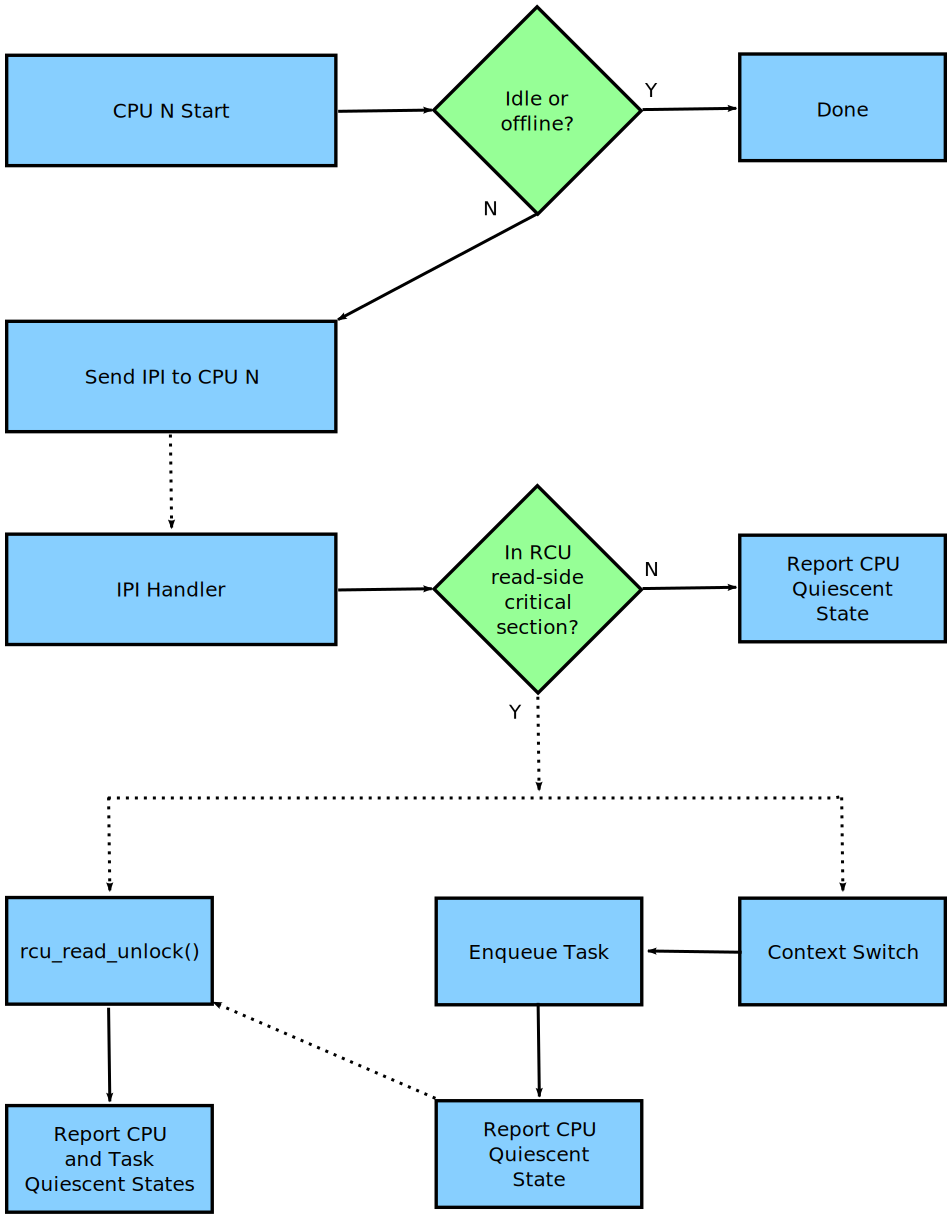
\includegraphics{rcu/design/ExpRCUFlow}}
\end{center}

The solid arrows denote direct action, for example, a function call.
The dotted arrows denote indirect action, for example, an IPI
or a state that is reached after some time.

If a given CPU is offline or idle, \co{synchronize_rcu_expedited()}
will ignore it because idle and offline CPUs are already residing
in quiescent states.
Otherwise, the expedited grace period will use
\co{smp_call_function_single()} to send the CPU an IPI, which
is handled by \co{rcu_exp_handler()}.

However, because this is preemptible RCU, \co{rcu_exp_handler()}
can check to see if the CPU is currently running in an RCU read-side
critical section.
If not, the handler can immediately report a quiescent state.
Otherwise, it sets flags so that the outermost \co{rcu_read_unlock()}
invocation will provide the needed quiescent-state report.
This flag-setting avoids the previous forced preemption of all
CPUs that might have RCU read-side critical sections.
In addition, this flag-setting is done so as to avoid increasing
the overhead of the common-case fastpath through the scheduler.

Again because this is preemptible RCU, an RCU read-side critical section
can be preempted.
When that happens, RCU will enqueue the task, which will the continue to
block the current expedited grace period until it resumes and finds its
outermost \co{rcu_read_unlock()}.
The CPU will report a quiescent state just after enqueuing the task because
the CPU is no longer blocking the grace period.
It is instead the preempted task doing the blocking.
The list of blocked tasks is managed by \co{rcu_preempt_ctxt_queue()},
which is called from \co{rcu_preempt_note_context_switch()}, which
in turn is called from \co{rcu_note_context_switch()}, which in
turn is called from the scheduler.


\QuickQuiz{
  Why not just have the expedited grace period check the state of all
  the CPUs?
  After all, that would avoid all those real-time-unfriendly
  IPIs.
}\QuickQuizAnswer{
  Because we want the RCU read-side critical sections to run fast,
  which means no memory barriers.
  Therefore, it is not possible to
  safely check the state from some other CPU\@.
  And even if it was
  possible to safely check the state, it would still be necessary to
  IPI the CPU to safely interact with the upcoming
  \co{rcu_read_unlock()} invocation, which means that the remote state
  testing would not help the worst-case latency that real-time
  applications care about.

  One way to prevent your real-time application from getting hit with
  these IPIs is to build your kernel with \co{CONFIG_NO_HZ_FULL=y}.
  RCU
  would then perceive the CPU running your application as being idle,
  and it would be able to safely detect that state without needing to
  IPI the CPU\@.
}\QuickQuizEnd

Please note that this is just the overall flow:
Additional complications
can arise due to races with CPUs going idle or offline, among other
things.

\subsection{RCU-sched Expedited Grace Periods}

\co{CONFIG_PREEMPTION=n} kernels implement RCU-sched.
The overall flow of
the handling of a given CPU by an RCU-sched expedited grace period is
shown in the following diagram:

\begin{center}
\resizebox{.6\columnwidth}{!}{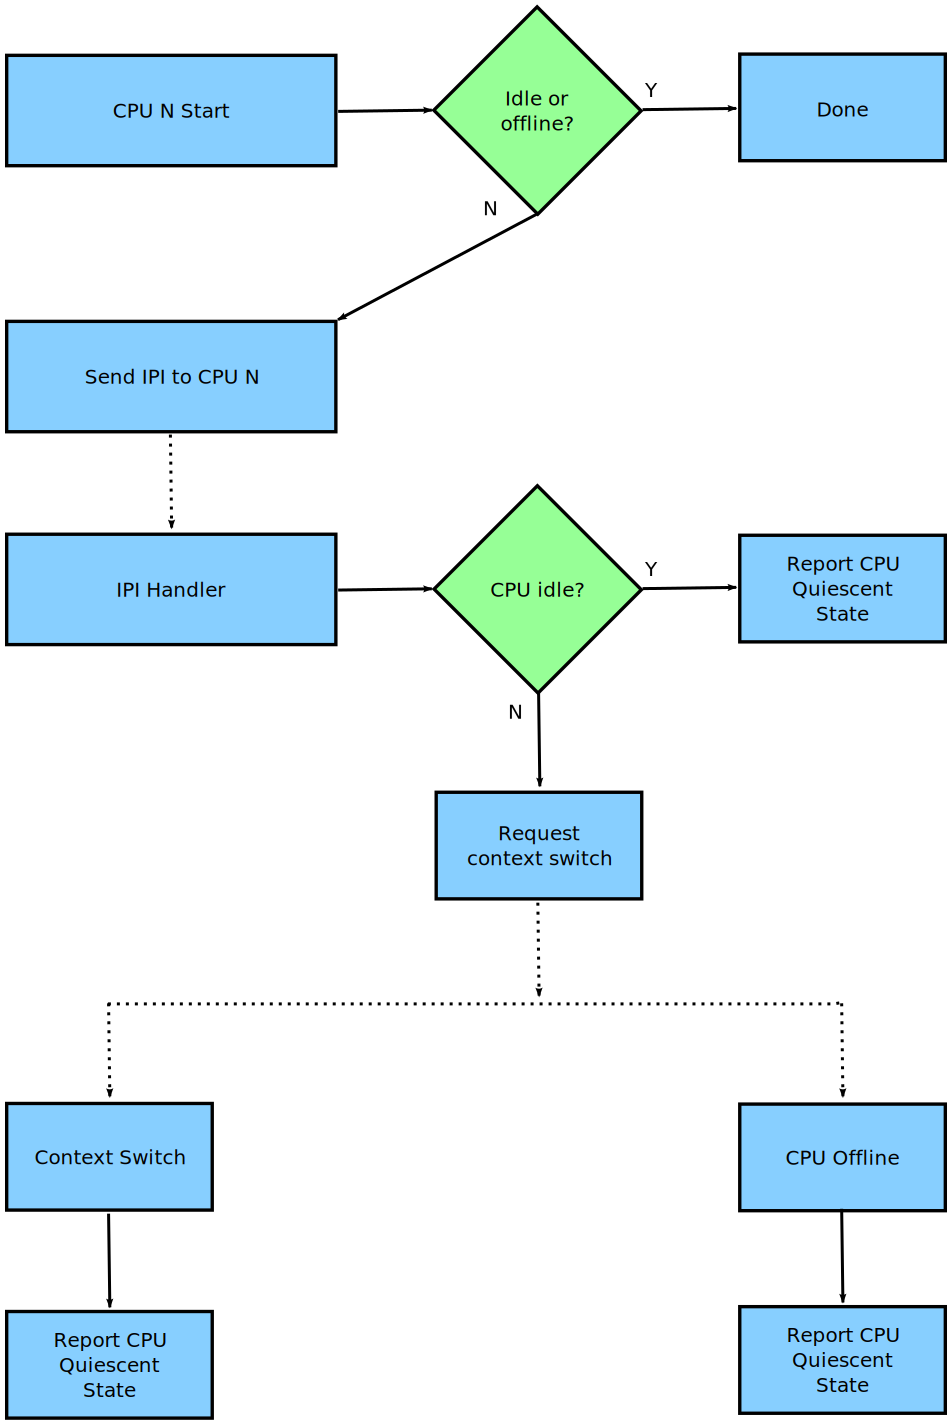
\includegraphics{rcu/design/ExpSchedFlow}}
\end{center}

As with RCU-preempt, RCU-sched's \co{synchronize_rcu_expedited()} ignores
offline and idle CPUs, again because they are in remotely detectable
quiescent states.
However, because the \co{rcu_read_lock_sched()} and
\co{rcu_read_unlock_sched()} leave no trace of their invocation, in
general it is not possible to tell whether or not the current CPU is in
an RCU read-side critical section.
The best that RCU-sched's
\co{rcu_exp_handler()} can do is to check for idle, on the off-chance
that the CPU went idle while the IPI was in flight.
If the CPU is idle,
then \co{rcu_exp_handler()} reports the quiescent state.

Otherwise, the handler forces a future context switch by setting the
\co{NEED_RESCHED} flag of the current task's thread flag and the CPU preempt
counter.
At the time of the context switch, the CPU reports the
quiescent state. Should the CPU go offline first, it will report the
quiescent state at that time.


\subsection{Expedited Grace Period and CPU Hotplug}

The expedited nature of expedited grace periods require a much tighter
interaction with CPU hotplug operations than is required for normal
grace periods.
In addition, attempting to IPI offline CPUs will result
in splats, but failing to IPI online CPUs can result in too-short grace
periods.
Neither option is acceptable in production kernels.

The interaction between expedited grace periods and CPU hotplug
operations is carried out at several levels:

\begin{enumerate}
\item The number of CPUs that have ever been online is tracked by the
   \co{rcu_state} structure's \co{->ncpus} field.
   The \co{rcu_state}
   structure's \co{->ncpus_snap} field tracks the number of CPUs that
   have ever been online at the beginning of an RCU expedited grace
   period.
   Note that this number never decreases, at least in the
   absence of a time machine.

\item The identities of the CPUs that have ever been online is tracked by
   the \co{rcu_node} structure's \co{->expmaskinitnext} field.
   The
   \co{rcu_node} structure's \co{->expmaskinit} field tracks the
   identities of the CPUs that were online at least once at the
   beginning of the most recent RCU expedited grace period.
   The
   \co{rcu_state} structure's \co{->ncpus} and \co{->ncpus_snap} fields are
   used to detect when new CPUs have come online for the first time,
   that is, when the \co{rcu_node} structure's \co{->expmaskinitnext}
   field has changed since the beginning of the last RCU expedited grace
   period, which triggers an update of each \co{rcu_node} structure's
   \co{->expmaskinit} field from its \co{->expmaskinitnext} field.

\item Each \co{rcu_node} structure's \co{->expmaskinit} field is used to
   initialize that structure's \co{->expmask} at the beginning of each
   RCU expedited grace period.
   This means that only those CPUs that have
   been online at least once will be considered for a given grace
   period.

\item Any CPU that goes offline will clear its bit in its leaf \co{rcu_node}
   structure's \co{->qsmaskinitnext} field, so any CPU with that bit
   clear can safely be ignored.
   However, it is possible for a CPU coming
   online or going offline to have this bit set for some time while
   \co{cpu_online} returns \co{false}.

\item For each non-idle CPU that RCU believes is currently online, the
   grace period invokes \co{smp_call_function_single()}.
   If this
   succeeds, the CPU was fully online.
   Failure indicates that the CPU is
   in the process of coming online or going offline, in which case it is
   necessary to wait for a short time period and try again.
   The purpose
   of this wait (or series of waits, as the case may be) is to permit a
   concurrent CPU-hotplug operation to complete.

\item In the case of RCU-sched, one of the last acts of an outgoing CPU is
   to invoke \co{rcutree_report_cpu_dead()}, which reports a quiescent state for
   that CPU\@.
   However, this is likely paranoia-induced redundancy.
\end{enumerate}

\QuickQuiz{
  Why all the dancing around with multiple counters and masks tracking
  CPUs that were once online? Why not just have a single set of masks
  tracking the currently online CPUs and be done with it?
}\QuickQuizAnswer{
  Maintaining single set of masks tracking the online CPUs \emph{sounds}
  easier, at least until you try working out all the race conditions
  between grace-period initialization and CPU-hotplug operations.
  For
  example, suppose initialization is progressing down the tree while a
  CPU-offline operation is progressing up the tree.
  This situation can
  result in bits set at the top of the tree that have no counterparts
  at the bottom of the tree.
  Those bits will never be cleared, which
  will result in grace-period hangs.
  In short, that way lies madness,
  to say nothing of a great many bugs, hangs, and deadlocks.
  In contrast, the current multi-mask multi-counter scheme ensures that
  grace-period initialization will always see consistent masks up and
  down the tree, which brings significant simplifications over the
  single-mask method.

  This is an instance of
  % dead link (or need login account?): http://www.cs.columbia.edu/~library/TR-repository/reports/reports-1992/cucs-039-92.ps.gz
  % Synthesis: an efficient implementation of fundamental operating system services
  % Wikipedia uses this link: https://www.scs.stanford.edu/nyu/04fa/sched/readings/synthesis.pdf
  % At ACM: https://dl.acm.org/doi/10.5555/143219
  \href{https://web.archive.org/web/20160622054529/http://www.cs.columbia.edu/~library/TR-repository/reports/reports-1992/cucs-039-92.ps.gz}
  {deferring work in order to avoid synchronization}.
  Lazily recording CPU-hotplug events at the beginning of the next
  grace period greatly simplifies maintenance of the CPU-tracking
  bitmasks in the \co{rcu_node} tree.
}\QuickQuizEnd


\subsection{Expedited Grace Period Refinements}

\subsubsection{Idle-CPU Checks}

Each expedited grace period checks for idle CPUs when initially forming
the mask of CPUs to be IPIed and again just before IPIing a CPU (both
checks are carried out by \co{sync_rcu_exp_select_cpus()}).
If the CPU is
idle at any time between those two times, the CPU will not be IPIed.
Instead, the task pushing the grace period forward will include the idle
CPUs in the mask passed to \co{rcu_report_exp_cpu_mult()}.

For RCU-sched, there is an additional check:
If the IPI has interrupted
the idle loop, then \co{rcu_exp_handler()} invokes
\co{rcu_report_exp_rdp()} to report the corresponding quiescent state.

For RCU-preempt, there is no specific check for idle in the IPI handler
(\co{rcu_exp_handler()}), but because RCU read-side critical sections are
not permitted within the idle loop, if \co{rcu_exp_handler()} sees that
the CPU is within RCU read-side critical section, the CPU cannot
possibly be idle.
Otherwise, \co{rcu_exp_handler()} invokes
\co{rcu_report_exp_rdp()} to report the corresponding quiescent state,
regardless of whether or not that quiescent state was due to the CPU
being idle.

In summary, RCU expedited grace periods check for idle when building the
bitmask of CPUs that must be IPIed, just before sending each IPI, and
(either explicitly or implicitly) within the IPI handler.

\subsubsection{Batching via Sequence Counter}

If each grace-period request was carried out separately, expedited grace
periods would have abysmal scalability and problematic high-load
characteristics.
Because each grace-period operation can serve an
unlimited number of updates, it is important to \emph{batch} requests, so
that a single expedited grace-period operation will cover all requests
in the corresponding batch.

This batching is controlled by a sequence counter named
\co{->expedited_sequence} in the \co{rcu_state} structure.
This counter
has an odd value when there is an expedited grace period in progress and
an even value otherwise, so that dividing the counter value by two gives
the number of completed grace periods.
During any given update request,
the counter must transition from even to odd and then back to even, thus
indicating that a grace period has elapsed.
Therefore, if the initial
value of the counter is \co{s}, the updater must wait until the counter
reaches at least the value \co{(s+3)&~0x1}.
This counter is managed by
the following access functions:

\begin{enumerate}
\item \co{rcu_exp_gp_seq_start()}, which marks the start of an expedited
   grace period.
\item \co{rcu_exp_gp_seq_end()}, which marks the end of an expedited grace
   period.
\item \co{rcu_exp_gp_seq_snap()}, which obtains a snapshot of the counter.
\item \co{rcu_exp_gp_seq_done()}, which returns \co{true} if a full expedited
   grace period has elapsed since the corresponding call to
   \co{rcu_exp_gp_seq_snap()}.
\end{enumerate}

Again, only one request in a given batch need actually carry out a
grace-period operation, which means there must be an efficient way to
identify which of many concurrent requests will initiate the grace
period, and that there be an efficient way for the remaining requests to
wait for that grace period to complete.
However, that is the topic of
the next section.

\subsubsection{Funnel Locking and Wait/Wakeup}

The natural way to sort out which of a batch of updaters will initiate
the expedited grace period is to use the \co{rcu_node} combining tree, as
implemented by the \co{exp_funnel_lock()} function.
The first updater
corresponding to a given grace period arriving at a given \co{rcu_node}
structure records its desired grace-period sequence number in the
\co{->exp_seq_rq} field and moves up to the next level in the tree.
Otherwise, if the \co{->exp_seq_rq} field already contains the sequence
number for the desired grace period or some later one, the updater
blocks on one of four wait queues in the \co{->exp_wq[]} array, using the
second-from-bottom and third-from bottom bits as an index.
An
\co{->exp_lock} field in the \co{rcu_node} structure synchronizes access
to these fields.

An empty \co{rcu_node} tree is shown in the following diagram, with the
white cells representing the \co{->exp_seq_rq} field and the red cells
representing the elements of the \co{->exp_wq[]} array.

\begin{center}
\resizebox{\columnwidth}{!}{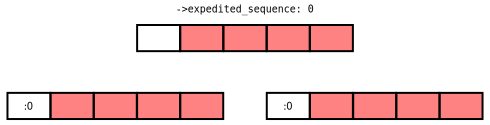
\includegraphics{rcu/design/Funnel0}}
\end{center}

The next diagram shows the situation after the arrival of Task~A and
Task~B at the leftmost and rightmost leaf \co{rcu_node} structures,
respectively.
The current value of the \co{rcu_state} structure's
\co{->expedited_sequence} field is zero, so adding three and clearing the
bottom bit results in the value two, which both tasks record in the
\co{->exp_seq_rq} field of their respective \co{rcu_node} structures:

\begin{center}
\resizebox{\columnwidth}{!}{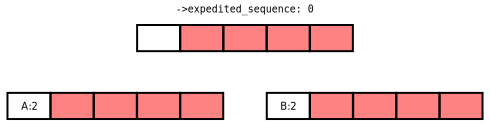
\includegraphics{rcu/design/Funnel1}}
\end{center}

Each of Tasks~A and~B will move up to the root \co{rcu_node} structure.
Suppose that Task~A wins, recording its desired grace-period sequence
number and resulting in the state shown below:

\begin{center}
\resizebox{\columnwidth}{!}{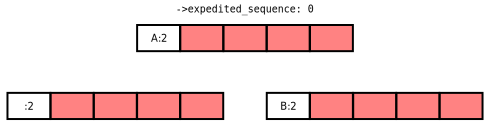
\includegraphics{rcu/design/Funnel2}}
\end{center}

Task~A now advances to initiate a new grace period, while Task~B moves
up to the root \co{rcu_node} structure, and, seeing that its desired
sequence number is already recorded, blocks on \co{->exp_wq[1]}.

\QuickQuiz{
  Why \co{->exp_wq[1]}?
  Given that the value of these tasks' desired
  sequence number is two, so shouldn't they instead block on
  \co{->exp_wq[2]}?
}\QuickQuizAnswer{
  No.
  Recall that the bottom bit of the desired sequence number indicates
  whether or not a grace period is currently in progress.
  It is
  therefore necessary to shift the sequence number right one bit
  position to obtain the number of the grace period.
  This results in
  \co{->exp_wq[1]}.
}\QuickQuizEnd

If Tasks~C and~D also arrive at this point, they will compute the same
desired grace-period sequence number, and see that both leaf
\co{rcu_node} structures already have that value recorded.
They will
therefore block on their respective \co{rcu_node} structures'
\co{->exp_wq[1]} fields, as shown below:

\begin{center}
\resizebox{\columnwidth}{!}{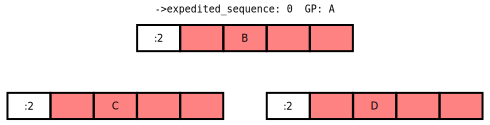
\includegraphics{rcu/design/Funnel3}}
\end{center}

Task~A now acquires the \co{rcu_state} structure's \co{->exp_mutex} and
initiates the grace period, which increments \co{->expedited_sequence}.
Therefore, if Tasks~E and~F arrive, they will compute a desired sequence
number of 4 and will record this value as shown below:

\begin{center}
\resizebox{\columnwidth}{!}{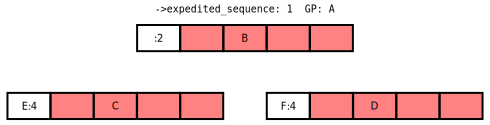
\includegraphics{rcu/design/Funnel4}}
\end{center}

Tasks~E and~F will propagate up the \co{rcu_node} combining tree, with
Task~F blocking on the root \co{rcu_node} structure and Task~E wait for
Task~A to finish so that it can start the next grace period.
The
resulting state is as shown below:

\begin{center}
\resizebox{\columnwidth}{!}{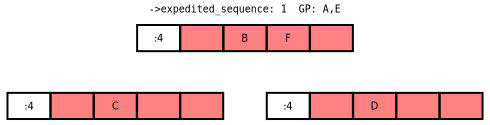
\includegraphics{rcu/design/Funnel5}}
\end{center}

Once the grace period completes, Task~A starts waking up the tasks
waiting for this grace period to complete, increments the
\co{->expedited_sequence}, acquires the \co{->exp_wake_mutex} and then
releases the \co{->exp_mutex}.
This results in the following state:

\begin{center}
\resizebox{\columnwidth}{!}{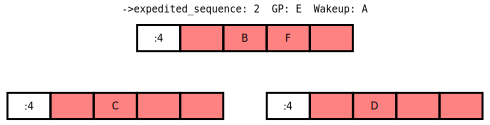
\includegraphics{rcu/design/Funnel6}}
\end{center}

Task~E can then acquire \co{->exp_mutex} and increment
\co{->expedited_sequence} to the value three.
If new tasks~G and~H arrive
and moves up the combining tree at the same time, the state will be as
follows:

\begin{center}
\resizebox{\columnwidth}{!}{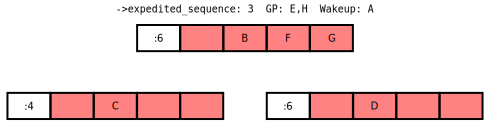
\includegraphics{rcu/design/Funnel7}}
\end{center}

Note that three of the root \co{rcu_node} structure's waitqueues are now
occupied.
However, at some point, Task~A will wake up the tasks blocked
on the \co{->exp_wq} waitqueues, resulting in the following state:

\begin{center}
\resizebox{\columnwidth}{!}{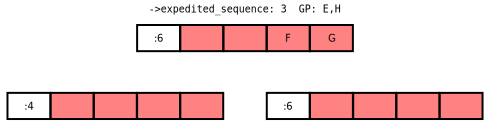
\includegraphics{rcu/design/Funnel8}}
\end{center}

Execution will continue with Tasks~E and~H completing their grace
periods and carrying out their wakeups.

\QuickQuiz{
  What happens if Task~A takes so long to do its wakeups that Task~E's
  grace period completes?
}\QuickQuizAnswer{
  Then Task~E will block on the \co{->exp_wake_mutex}, which will also
  prevent it from releasing \co{->exp_mutex}, which in turn will prevent
  the next grace period from starting.
  This last is important in
  preventing overflow of the \co{->exp_wq[]} array.
}\QuickQuizEnd

\subsubsection{Use of Workqueues}

In earlier implementations, the task requesting the expedited grace
period also drove it to completion.
This straightforward approach had
the disadvantage of needing to account for POSIX signals sent to user
tasks, so more recent implementations use the Linux kernel's
workqueues (see \path{Documentation/core-api/workqueue.rst}).

The requesting task still does counter snapshotting and funnel-lock
processing, but the task reaching the top of the funnel lock does a
\co{schedule_work()} (from \co{_synchronize_rcu_expedited()} so that a
workqueue kthread does the actual grace-period processing.
Because
workqueue kthreads do not accept POSIX signals, grace-period-wait
processing need not allow for POSIX signals.
In addition, this approach
allows wakeups for the previous expedited grace period to be overlapped
with processing for the next expedited grace period.
Because there are
only four sets of waitqueues, it is necessary to ensure that the
previous grace period's wakeups complete before the next grace period's
wakeups start.
This is handled by having the \co{->exp_mutex} guard
expedited grace-period processing and the \co{->exp_wake_mutex} guard
wakeups.
The key point is that the \co{->exp_mutex} is not released until
the first wakeup is complete, which means that the \co{->exp_wake_mutex}
has already been acquired at that point.
This approach ensures that the
previous grace period's wakeups can be carried out while the current
grace period is in process, but that these wakeups will complete before
the next grace period starts.
This means that only three waitqueues are
required, guaranteeing that the four that are provided are sufficient.

\subsubsection{Stall Warnings}

Expediting grace periods does nothing to speed things up when RCU
readers take too long, and therefore expedited grace periods check for
stalls just as normal grace periods do.

\QuickQuiz{
  But why not just let the normal grace-period machinery detect the
  stalls, given that a given reader must block both normal and
  expedited grace periods?
}\QuickQuizAnswer{
  Because it is quite possible that at a given time there is no normal
  grace period in progress, in which case the normal grace period
  cannot emit a stall warning.
}\QuickQuizEnd

The \co{synchronize_sched_expedited_wait()} function loops waiting for
the expedited grace period to end, but with a timeout set to the current
RCU CPU stall-warning time.
If this time is exceeded, any CPUs or
\co{rcu_node} structures blocking the current grace period are printed.
Each stall warning results in another pass through the loop, but the
second and subsequent passes use longer stall times.

\subsubsection{Mid-boot operation}

The use of workqueues has the advantage that the expedited grace-period
code need not worry about POSIX signals.
Unfortunately, it has the
corresponding disadvantage that workqueues cannot be used until they are
initialized, which does not happen until some time after the scheduler
spawns the first task.
Given that there are parts of the kernel that
really do want to execute grace periods during this mid-boot ``dead
zone'', expedited grace periods must do something else during this time.

What they do is to fall back to the old practice of requiring that the
requesting task drive the expedited grace period, as was the case before
the use of workqueues.
However, the requesting task is only required to
drive the grace period during the mid-boot dead zone.
Before mid-boot, a
synchronous grace period is a no-op. Some time after mid-boot,
workqueues are used.

Non-expedited non-SRCU synchronous grace periods must also operate
normally during mid-boot.
This is handled by causing non-expedited grace
periods to take the expedited code path during mid-boot.

The current code assumes that there are no POSIX signals during the
mid-boot dead zone.
However, if an overwhelming need for POSIX signals
somehow arises, appropriate adjustments can be made to the expedited
stall-warning code.
One such adjustment would reinstate the
pre-workqueue stall-warning checks, but only during the mid-boot dead
zone.

With this refinement, synchronous grace periods can now be used from
task context pretty much any time during the life of the kernel.
That
is, aside from some points in the suspend, hibernate, or shutdown code
path.

\subsection{Summary}

Expedited grace periods use a sequence-number approach to promote
batching, so that a single grace-period operation can serve numerous
requests.
A funnel lock is used to efficiently identify the one task out
of a concurrent group that will request the grace period.
All members of
the group will block on waitqueues provided in the \co{rcu_node}
structure.
The actual grace-period processing is carried out by a
workqueue.

CPU-hotplug operations are noted lazily in order to prevent the need for
tight synchronization between expedited grace periods and CPU-hotplug
operations.
The dyntick-idle counters are used to avoid sending IPIs to
idle CPUs, at least in the common case. RCU-preempt and RCU-sched use
different IPI handlers and different code to respond to the state
changes carried out by those handlers, but otherwise use common code.

Quiescent states are tracked using the \co{rcu_node} tree, and once all
necessary quiescent states have been reported, all tasks waiting on this
expedited grace period are awakened.
A pair of mutexes are used to allow
one grace period's wakeups to proceed concurrently with the next grace
period's processing.

This combination of mechanisms allows expedited grace periods to run
reasonably efficiently.
However, for non-time-critical tasks, normal
grace periods should be used instead because their longer duration
permits much higher degrees of batching, and thus much lower per-request
overheads.
